\section{Durchführung}
\label{sec:Durchführung}
In der Abbildung \ref{fig:aufbau} ist der Versuchsaufbau schematisch skizziert. Es sind zwei verschiebbaren Meßuhren zu erkennen, die die Auslenkung messen. Die Probekörper werden einseitig an der Position C 
befestigt und beidseitig an den Positionen A und B. Die Durchbiegung erfolgt erst, wenn das Gewicht angehängt wird. Bei der einseitigen Einspannung wird das Gewicht am Ende der Stabes angehängt und im Gegensatz 
zu der einseitigen, wird das Gewicht mittig bei der beidseitigen Einspannung angehängt.
Außerdem ist auch noch eine Längenskala an der Apparatur abgebildet. Diese dient zur Messung der Biegung an verschiedenen Stellen. 
Es wird davon ausgegangen, dass die Stäbe nicht gerade sind und deswegen soll eine Nullmessung ohne Last durchgeführt werden. 
\begin{figure}[h!]
	\centering
	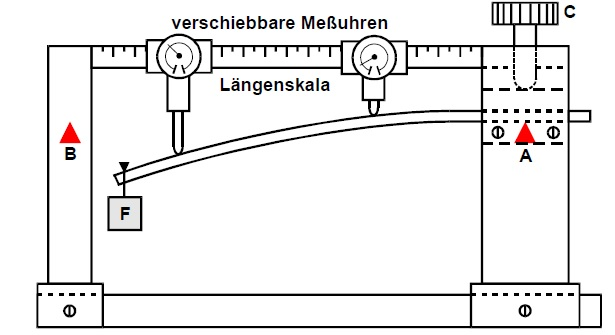
\includegraphics[width=0.7\linewidth]{Aufbau.jpg}
	\caption{Aufbau der Apparatur zur Messung der elastischen Stäbe, \cite[6]{anleitung103}.}
	\label{fig:aufbau}
\end{figure}
Es werden Stäbe mit einem zylindrischen und quadratischen Querschnitt verwendet, die aus verschiedenen Materialien bestehen. Diese beiden werden zuerst gewogen, danach wird mit einer 
Schieblehre $10$ mal die Breite und die Höhe vermessen. 

Anschließend wird der Stab einseitig an der Position C eingespannt, und mit Hilfe der Meßuhren wird an $10$ Stellen die Durchbiegung gemessen.
Dabei ist $D_{0}(x)$ die Durchbiegung ohne Last, und $D_{\text{m}}(x)$ dann die Durchbiegung mit Gewicht. Die Werte werden in Abhängigkeit vom Abstand $x$ in einer Tabelle eingetragen. 
Die tatsächliche Durchbiegung berechnet sich mit:
\begin{equation*}
\label{eqn:Durchbiegung}
D(x) = D_{\text{m}}(x) - D_{0}(x).
\end{equation*}

Als nächstes wird das Verfahren analog für die beidseitige Einspannung wiederholt. Der Unterschied liegt jetzt nun daran, dass das Gewicht mittig angehängt wird und die Stäbe jeweils an den Positionen A  und B 
 befestigt werden. Es werden einmal von der rechten und linken Seite die Meßwerte notiert. Anschließend kann $D(x)$ bestimmt werden. 

Für die Messung der Durchbiegungen können die Messuhren auch so verwendet werden, dass sie bei jeder Messung neu eingestellt werden, sodass die Durchbiegung direkt ablesbar und deshalb keine Nullmessung erforderlich ist.